\documentclass[12pt]{article}
\usepackage{amsmath}
\usepackage{amssymb}
\usepackage[letterpaper,top=1.5in,bottom=1in,left=0.75in,right=0.75in,centering]{geometry}
%\usepackage{fancyhdr}
\usepackage{enumerate}
%\usepackage{lastpage}
\usepackage{multicol}
\usepackage{graphicx}

\reversemarginpar

%\pagestyle{fancy}
%\cfoot{}
%\lhead{Math 1560}\chead{Test \# 1}\rhead{May 18th, 2017}
%\rfoot{Total: 10 points}
%\chead{{\bf Name:}}
\newcommand{\points}[1]{\marginpar{\hspace{24pt}[#1]}}
\newcommand{\skipline}{\vspace{12pt}}
%\renewcommand{\headrulewidth}{0in}
\headheight 30pt

\newcommand{\di}{\displaystyle}
\newcommand{\abs}[1]{\lvert #1\rvert}
\newcommand{\len}[1]{\lVert #1\rVert}
\renewcommand{\i}{\mathbf{i}}
\renewcommand{\j}{\mathbf{j}}
\renewcommand{\k}{\mathbf{k}}
\newcommand{\R}{\mathbb{R}}
\newcommand{\aaa}{\mathbf{a}}
\newcommand{\bbb}{\mathbf{b}}
\newcommand{\ccc}{\mathbf{c}}
\newcommand{\dotp}{\boldsymbol{\cdot}}
\newcommand{\bbm}{\begin{bmatrix}}
\newcommand{\ebm}{\end{bmatrix}}                   
                  
\begin{document}


\author{Instructor: Sean Fitzpatrick}
\thispagestyle{empty}
\vglue1cm
\begin{center}
\emph{University of Lethbridge}\\
Department of Mathematics and Computer Science\\
{\bf MATH 1560 - Tutorial \#6}\\
Monday, February 26
\end{center}
\skipline \ \noindent \skipline

\vspace*{\fill}


Some additional practice (discuss the answers but don't write anything down):
\begin{enumerate}
\item Find the absolute (global) maximum and minimum values of the given function on the given interval:
\begin{enumerate}
\item $f(x) = x^2\sqrt{4-x^2}$, on $[-2,2]$.
\item $g(x) = x+\dfrac{3}{x}$, on $[1,5]$.
\item $h(x) = e^x\sin(x)$, on $[0,\pi]$
\end{enumerate}
\item Find all critical numbers for each function, and determine if each one is a local maximum, local minimum, or neither:
\begin{enumerate}
\item $f(x)=x^4-6x^2+4$
\item $g(x) = x^3\ln(x)$
\item $h(x) = x^2e^{-2x}$
\end{enumerate}
\end{enumerate}




\newpage
%\thispagestyle{empty}


\begin{enumerate}
\item Determine the global maximum and minimum values of the given function on the given interval. (Note: these values can occur at either a critical number or an end point.)
\begin{enumerate}
\item $f(x)=x^3-x^2$, on $[-1,2]$.

\vspace{2.5in}

\item $g(x) = 3x^{2/3}-2x$, on $[-1,8]$.

\vspace{2.5in}


\end{enumerate}

\item  Determine the intervals on which $f(x) = \dfrac{x^2+3}{x-1}$ is increasing and decreasing.

\newpage

\item Sketch the graph of $f(x) = (x-3)\sqrt{x}$. You will need the following:

\begin{itemize}
\item The domain of $f$, and any $x$ or $y$ intercepts.
\item The ``end behaviour'': are there any asymptotes?
\item The first derivative, location of any critical points (turning points), and intervals of increase/decrease.
\item The second derivative, location of any inflection points, and intervals of concave up/down.
\end{itemize}

\newpage


\item Extra fun: The graph of the \textit{derivative} of a \textbf{continuous} function $f$ is given below. From the graph, determine:
\begin{multicols}{2}
\begin{enumerate}
\item The intervals on which $f$ is increasing/decreasing.
\item The $x$-coordinates of any local maxima or minima.
\item The intervals on which $f$ is concave up/down.
\item The $x$-coordinates of any inflection points.
\item A rough graph of $f$, assuming that $f(0)=0$.
\end{enumerate}
\begin{center}
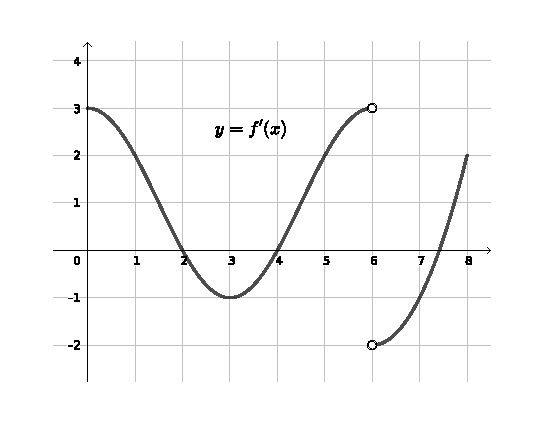
\includegraphics[width=\columnwidth]{Tut6-4}
\end{center}
\end{multicols}
  \end{enumerate}
\end{document}